\let\negmedspace\undefined
\let\negthickspace\undefined
\documentclass[journal]{IEEEtran}
\usepackage[a5paper, margin=10mm, onecolumn]{geometry}
%\usepackage{lmodern} % Ensure lmodern is loaded for pdflatex
\usepackage{tfrupee} % Include tfrupee package

\setlength{\headheight}{1cm} % Set the height of the header box
\setlength{\headsep}{0mm}     % Set the distance between the header box and the top of the text

\usepackage{gvv-book}
\usepackage{gvv}
\usepackage{cite}
\usepackage{amsmath,amssymb,amsfonts,amsthm}
\usepackage{algorithmic}
\usepackage{graphicx}
\usepackage{textcomp}
\usepackage{xcolor}
\usepackage{txfonts}
\usepackage{listings}
\usepackage{enumitem}
\usepackage{mathtools}
\usepackage{gensymb}
\usepackage{comment}
\usepackage[breaklinks=true]{hyperref}
\usepackage{tkz-euclide} 
\usepackage{listings}
% \usepackage{gvv}                                        
\def\inputGnumericTable{}                                 
\usepackage[latin1]{inputenc}                                
\usepackage{color}                                            
\usepackage{array}                                            
\usepackage{longtable}                                       
\usepackage{calc}                                             
\usepackage{multirow}                                         
\usepackage{hhline}                                           
\usepackage{ifthen}                                           
\usepackage{lscape}
\begin{document}

\bibliographystyle{IEEEtran}
\vspace{3cm}

\title{1.8.4}
\author{EE24BTECH11058 - P.Shiny Diavajna}
% \maketitle
% \newpage
% \bigskip
{\let\newpage\relax\maketitle}

\renewcommand{\thefigure}{\theenumi}
\renewcommand{\thetable}{\theenumi}
\setlength{\intextsep}{10pt} % Space between text and floats


\numberwithin{equation}{enumi}
\numberwithin{figure}{enumi}
\renewcommand{\thetable}{\theenumi}

\textbf{Question:} Find the coordinates of a point on Y axis which is at a distance of $5\sqrt2$ from the point $\vec{P}\brak{3,-2,5}$\\

   \solution
   \begin{table}[h!]    
     \centering
     \begin{tabular}[12pt]{ |c|c|}
    \hline
	\textbf{Symbol} & \textbf{Value} \\
    \hline
    $\vec{O}$ & Centre of the circle\\
    \hline 
    $3a$ & median of the triangle \\
    \hline
    $r$ & radius of the  circle \\

    \hline
    \end{tabular}

     \caption{Variables Used}
     \label{}
   \end{table}

   \begin{align*}
	   \vec{Q}=\vec{P}+\myvec{l\\m\\n} r\\
	   \myvec{0\\y\\0}=\myvec{3\\-2\\5} + \myvec{l\\m\\n} 5\sqrt2\\
	   l=\frac{-3}{5\sqrt2}\\
	   n=\frac{-5}{5\sqrt2}\\
           l^{2}+m^{2}+n^{2}=1\\
	   m=\pm \frac{4}{5\sqrt2}\\
	   y=-6 \brak{or} y=2\\
	   \vec{Q1}=\myvec{0\\-6\\0}  ,  \vec{Q2}=\myvec{0 \\2\\0}\\
   \end{align*}

    \begin{figure}[h]
    \centering
    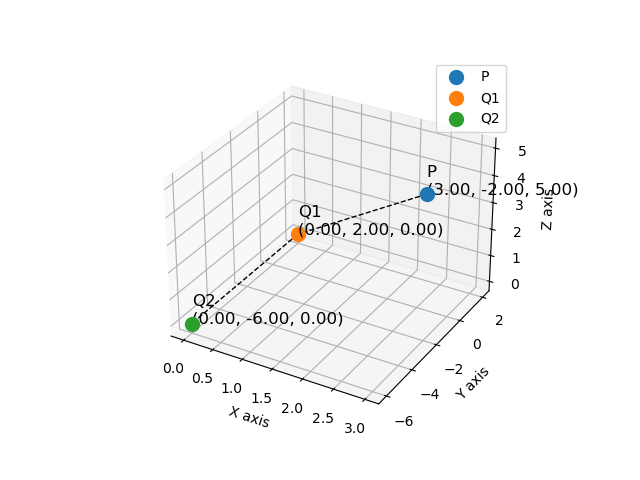
\includegraphics[width=\columnwidth]{figs/Figure_1.png}
    \caption{Plot of P, Q1 and Q2}
 \end{figure}


\end{document}
